\section {Meranie hustoty stavov v kove s disorderom metódou tunelovej spektroskopie}

V tejto kapitole uvedieme metódu merania hustoty stavov - tunelovú spektroskopiu.
Uvedieme tiež niekoľko vybraných experimentálnych výsledkov tejto metódy, ktoré sme prevzali z literatúry. Budú
motiváciou pre naše výpočty v nasledujúcich kapitolách.

Ako je ukázané na obrázku  \eqref{fig:schema}, experimentálna sústava pozostáva z dvoch kovov odelených tenkou vrstvou izolantu. Naľavo od izolantu je čistý
kov, ktorého hustota stavov sa dá v okolí Fermiho energie považovať za konštantu nezávislú od energie. t.j., nie je ovplyvnená javom Altshulera - Aronova. Napravo je {\it skúmaný kov} - kov s disorderom, ktorého
hustotu stavov chceme merať. Izolant tvorí potenciálovú bariéru, ktorá je dostatočne tenká na to, aby umožňovala slabé elektrónové tunelovanie z kovu do kovu.
Na sústavu sa priloží napätie  $U$, ktoré spôsobí, že z kovu do kovu tečie elektrónový tunelovací prúd $I(U)$. Meria sa volt-ampérová charakteristika $I(U)$ a diferenciálna vodivosť $dI(U)/dU$.
V nasledujúcich riadkoch stručne zhrnieme štandartnú teóriu tunelovacieho prúdu, ktorá umožňuje z nameranej diferenciálnej vodivosti $dI(U)/dU$ určiť hustotu stavov v skúmanom kove ako funkciu
elektrónovej energie $\E-\E_F$.


\begin{figure}
        \centering
        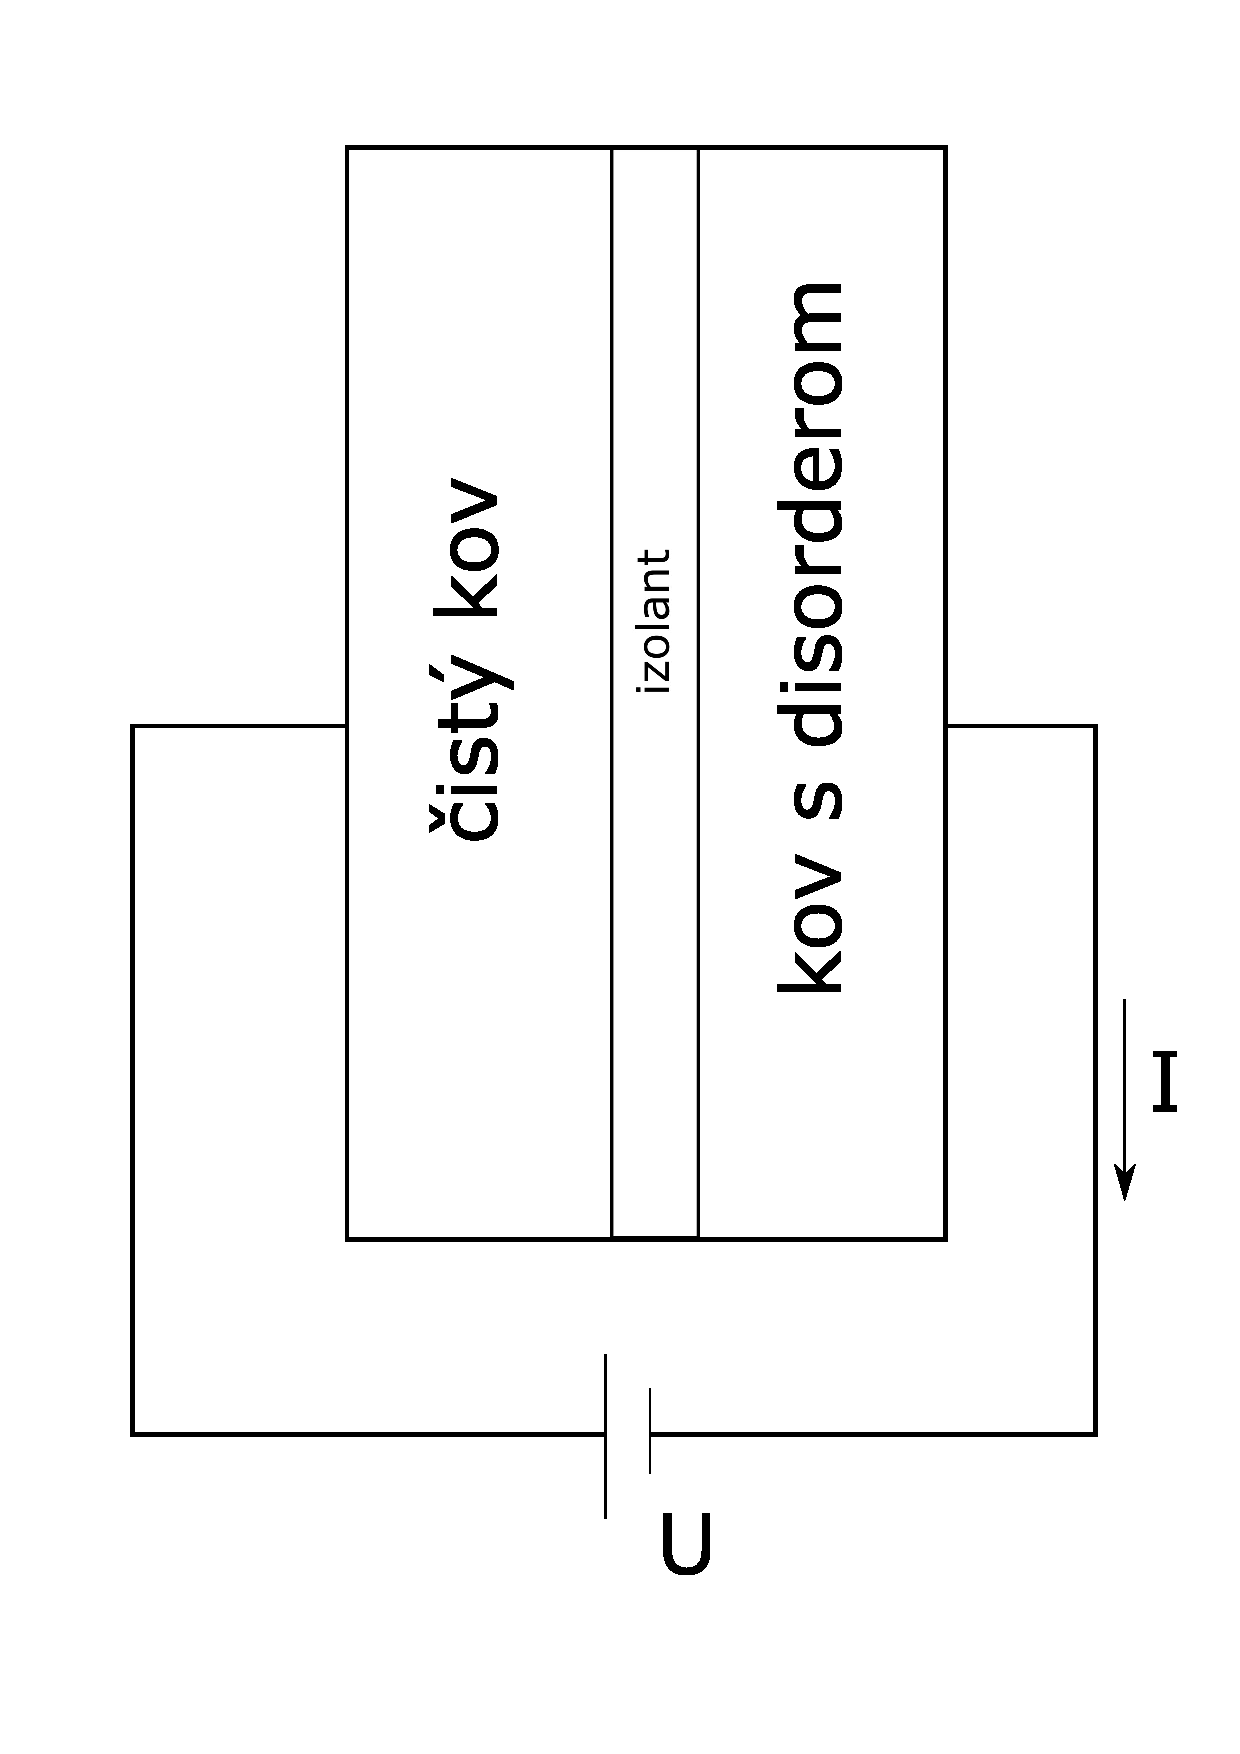
\includegraphics[origin=c,scale=0.4]{grafy/schema}
        \caption{Štruktúra kov-izolant-kov pre tunelovú spektroskopiu.}
        \label{fig:schema}
    \end{figure}
\begin{figure}
        \centering
        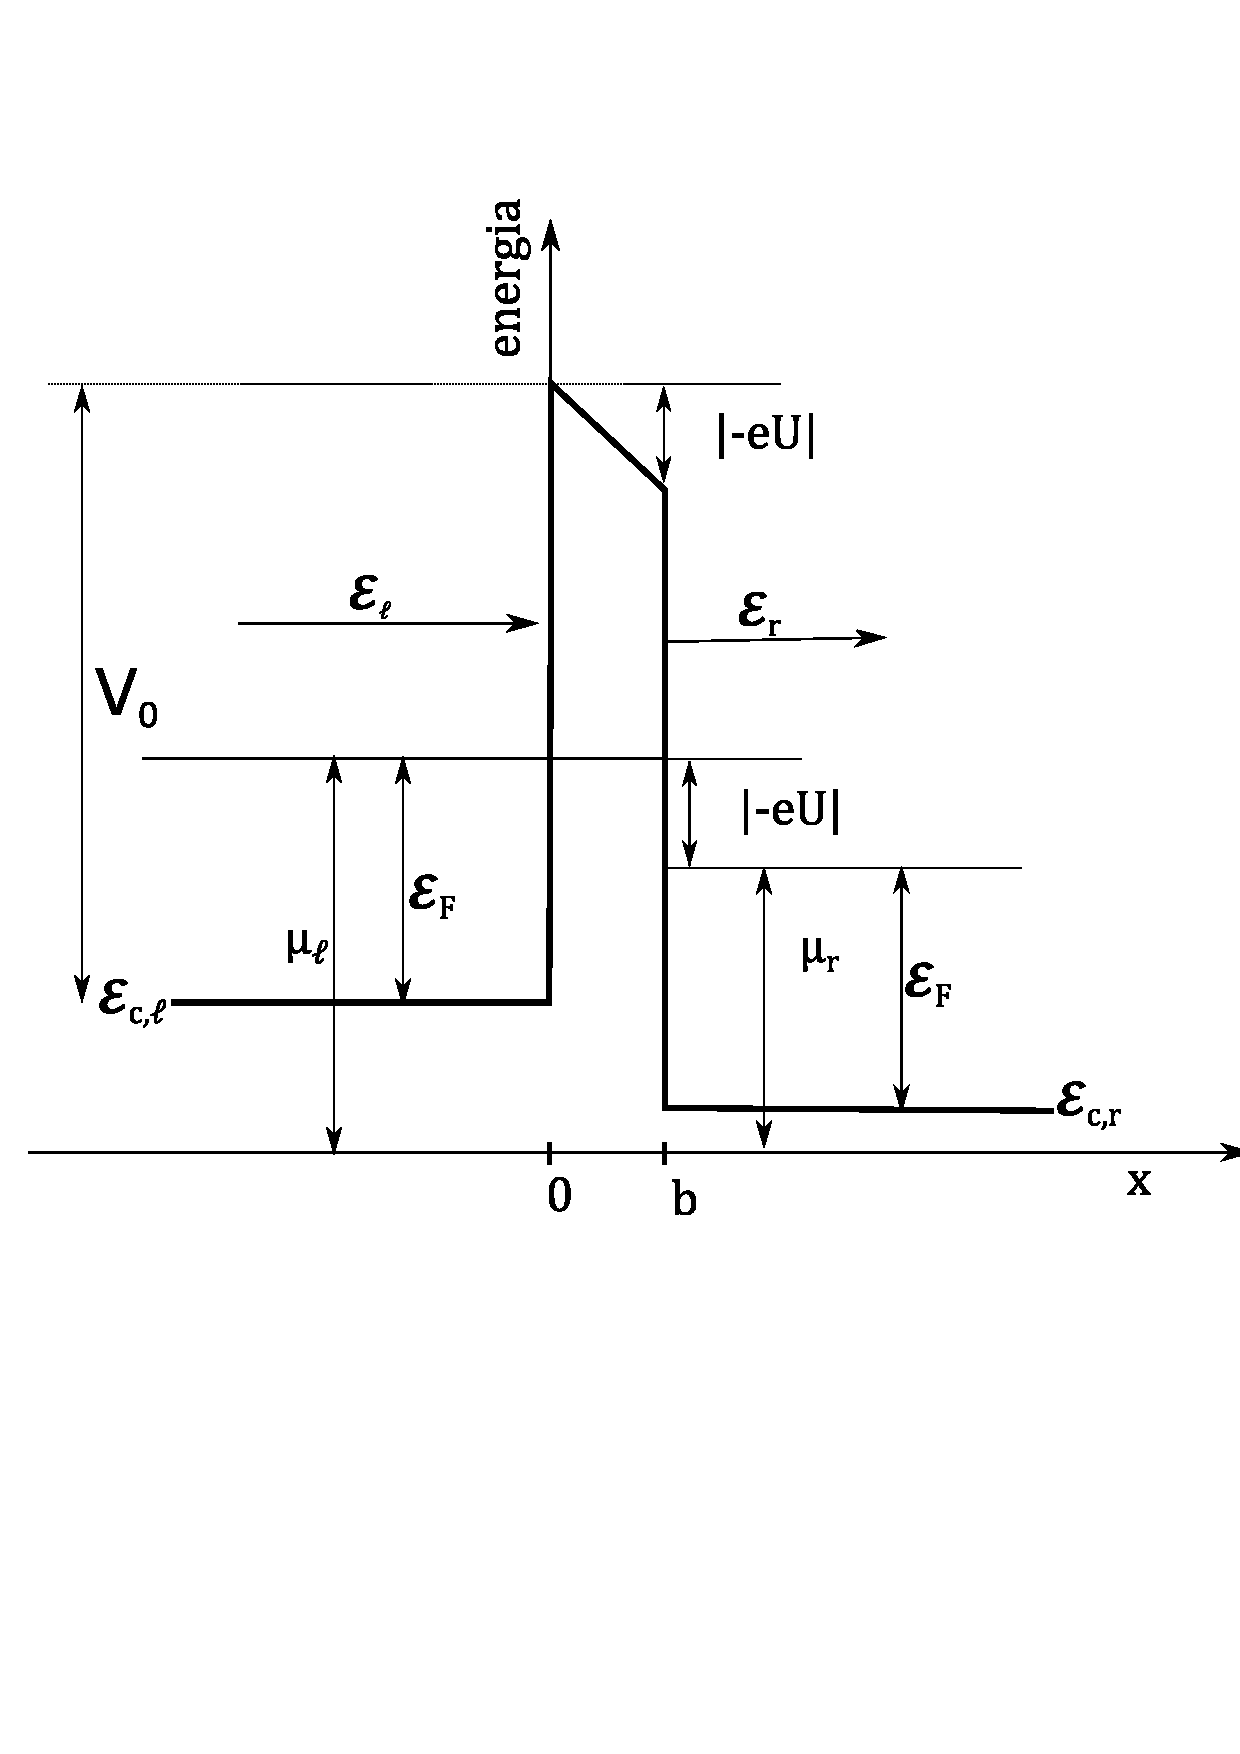
\includegraphics[origin=c,scale=0.5]{grafy/barier_v3}
        \caption{Pásový diagram  štruktúry kov-izolant-kov z predchádzajúceho obrázku. }
        \label{fig:barier_v3}
    \end{figure}
\begin{figure}
        \centering
        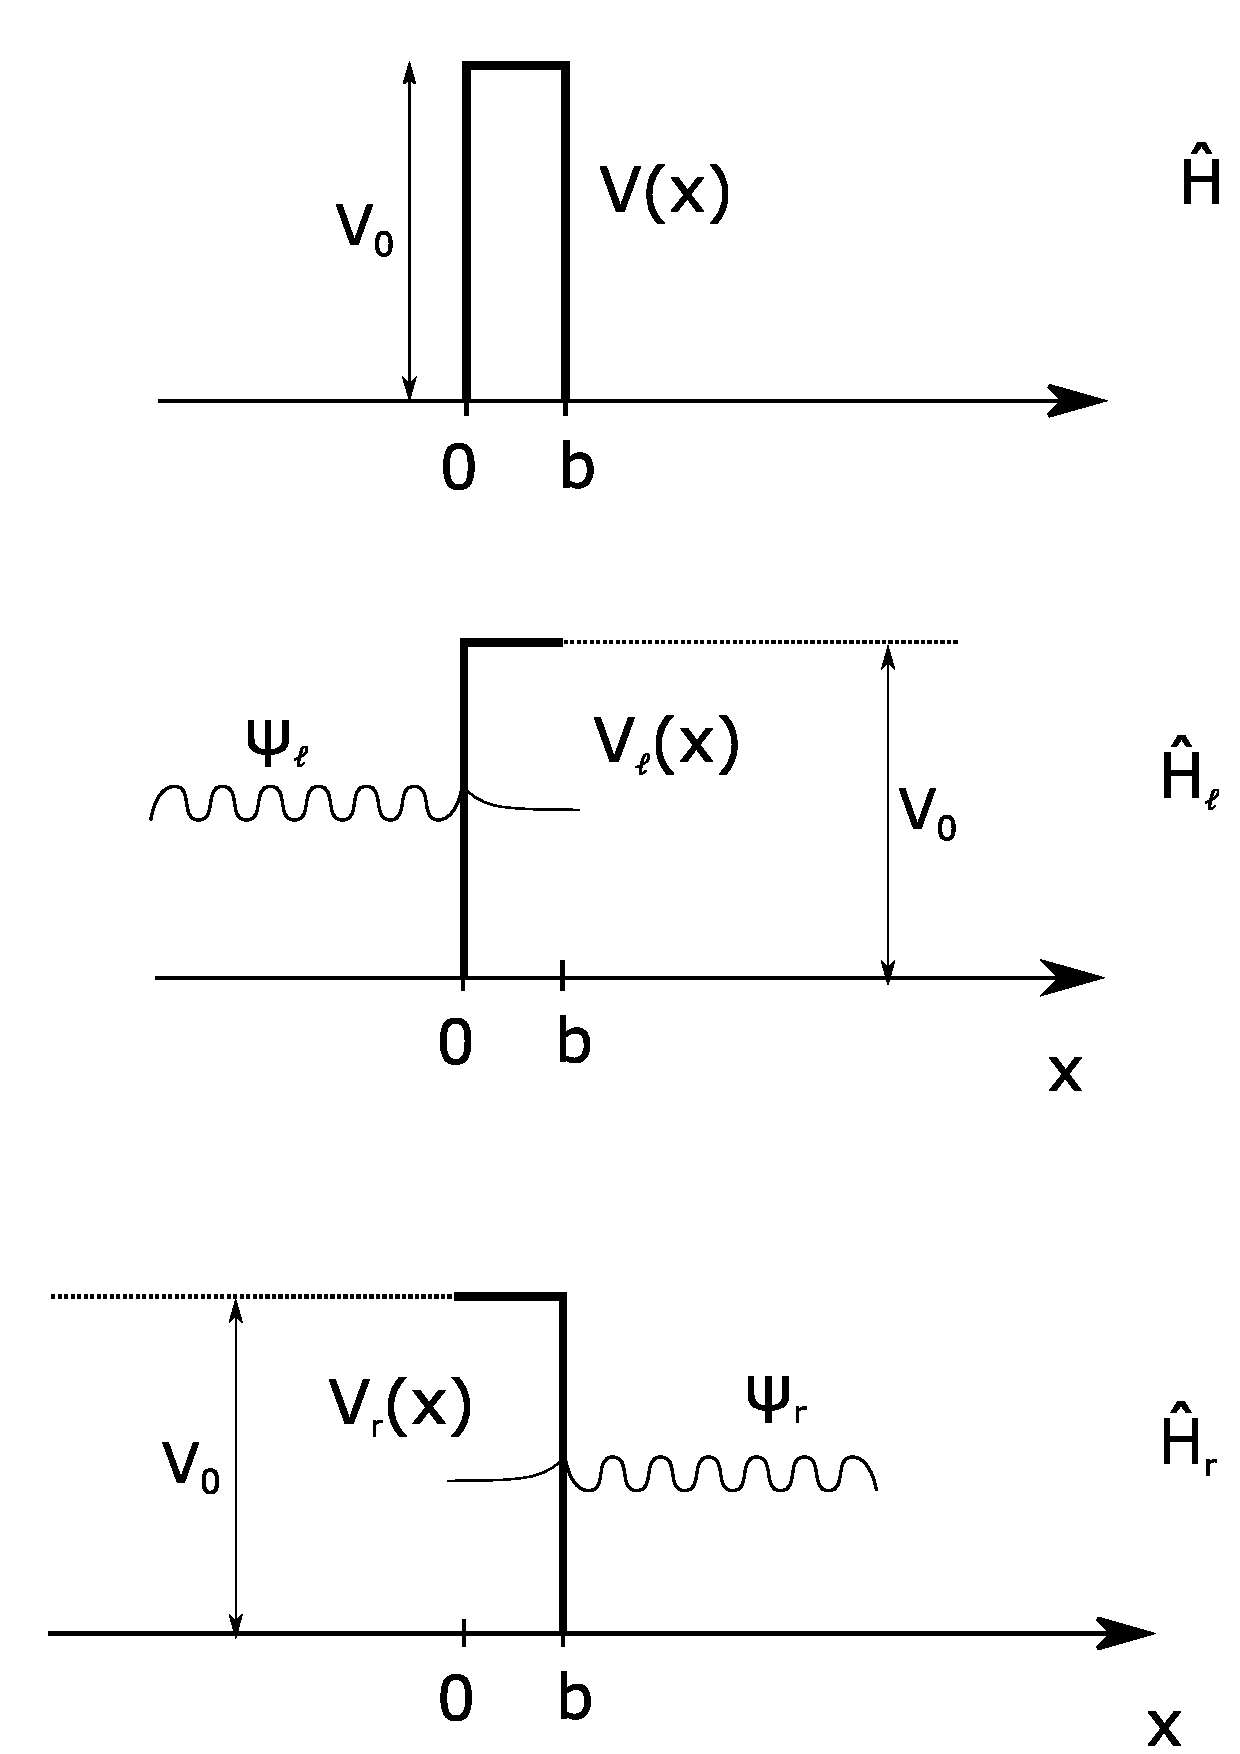
\includegraphics[origin=c,scale=0.5]{grafy/3bariers}
        \caption{Schématické znázornenie stavov $\psi_{l}(x)$ vľavo od bariéry a stavov $\psi_{r}(x)$ vpravo od bariéry podľa popisu v texte.}
        \label{fig:3bariers}
    \end{figure}
Na Obr. \eqref{fig:barier_v3}  je ukázaný pásový diagram štruktúry kov-izolant-kov, ktorý nám pomôže pri výpočte $I(U)$. Pre jednoduchosť uvažujeme dva rovnaké kovy s Fermiho energiou $\E_{F}$.
Energiu dna vodivostného pása označujeme $\E_{c,l}$ v kove vľavo od bariéry a $\E_{c,r}$ v kove vpravo od bariéry. Chemický potenciál elektrónov označujeme $\mu_{l}$ v kove vľavo a $\mu_{r}$ v kove vpravo.
Vlastnú hodnotu energie elektrónu v stave $l$ vľavo od bariéry označujeme ako $\E_{l}$ a vlastnú hodnotu energie elektrónu v stave $r$ vpravo od bariéry označujeme ako $\E_{r}$.  Izolant vytvára medzi kovmi energetickú bariéru výšky $V_{0}$, priložené napätie $U$ celé padá na bariéru a spôsobuje jej zošikmenie. Vidno, že $\mu_{l} - \mu_{r} = -eU$ a $\E_{c,l}  - \E_{c,r} = -eU$. Na obrázku sa predpokladá záporné $U$. Zdôraznime tiež, že energie $\E_{c,l}$, $\mu_{l}$,  a $\E_{l}$ aj energie $\E_{c,r}$, $\mu_{r}$,  a $\E_{r}$ sú na obrázku odčítané od tej istej nulovej hladiny.

Teraz definujme presnejšie, čo znamenajú pojmy stav $l$ a energia $\E_{l}$ vľavo od bariéry, a stav $r$ a energia $\E_{r}$ vpravo od bariéry.
K tomu nám pomôže obrázok \eqref{fig:3bariers}.
Hamiltonián $\hat{H}$ popisujúci pohyb elektrónu v celej štruktúre na obr. \eqref{fig:barier_v3} zapíšeme v tvare
\begin{equation}
 \hat{H}=-\frac{\hbar^2 \laplace }{2m}+V(x) \text{,}
\end{equation}
kde
\begin{equation}
 \label{eq:02potential_barrier}
 V(x)=
 \begin{cases}
    V_0,& \text{pre } 0<x<b\\
    0,              & \text{pre ostatné $x$}
\end{cases}\text{,}
\end{equation}
kde $b$ je šírka bariéry, $V_0$ je výška bariéry, a pre jednoduchosť neberieme do úvahy deformáciu bariéry spôsobenú priloženým napätím $U$.
Teraz namiesto bariéry opísanej potenciálom $V(x)$ uvažujme polonekonečnú bariéru opísanú potenciálom
\begin{equation}
 \label{eq:02potential_left}
 V_l(x)=
 \begin{cases}
    V_0,& \text{pre } 0<x\\
    0,              & \text{pre ostatné $x$}
\end{cases}\text{,}
\end{equation}
ktorý je ukázaný aj na \eqref{fig:3bariers}. Zodpovedajúci Hamiltoníán
\begin{equation}
 \hat{H_l}=-\frac{\hbar^2 \laplace }{2m}+V_l(x) \text{,}
\end{equation}
má vlastné funkcie $\psi_{l}(x)$ a vlastné energie $\E_{l}(x)$. Vlnové funkcie
$\psi_{l}(x)$ klesnú vo vnútri bariéry exponenciálne rýchlo na nulu. Preto o elektróne v stave
$\psi_{l}(x)$ s energiou $\E_{l}$ môžeme hovoriť ako o elektróne v stave $l$ vľavo od bariéry.
Podobne, uvažujme polonekonečnú bariéru opísanú potenciálom
 \begin{equation}
 \label{eq:02potential_right}
 V_r(x)=
 \begin{cases}
    V_0,& \text{pre } b>x\\
    0,              & \text{pre ostatné $x$}
\end{cases}\text{.}
\end{equation}
 Zodpovedajúci Hamiltoníán
\begin{equation}
 \hat{H_r}=-\frac{\hbar^2 \laplace }{2m}+V_r(x) \text{,}
\end{equation}
má vlastné funkcie $\psi_{r}(x)$ a vlastné energie $\E_{r}$. Podobne ako pre stavy $\psi_{l}(x)$,
o elektróne v stave
$\psi_{r}(x)$ s energiou $\E_{r}$ môžeme hovoriť ako o elektróne v stave $r$ vpravo od bariéry.

Uvažujme elektrón nachádzajúci sa v čase $t=0$ v stave $\psi_{l}(x)$, teda vľavo od bariéry. Keďže stav $\psi_{l}(x)$
nie je stacionárnym stavom Hamiltoniánu $\hat{H}$, existuje nenulová pravdepodobnosť $w_{l\to r}$,
že elektrón nachádzajúci sa v stave $\psi_l$ s energiou $E_r$ za jednotku času pretuneluje do niektorého zo stavov $\psi_r$ s energiou $E_r$.
Pravdepodobnosť $w_{l\to r}$ je daná Bardeenovou formulou
\begin{equation}
 \label{eq:02golden_rule}
 w_{l\to r}=\frac{2\pi}{\hbar} |\bra{\psi_r}\hat{H}-\E_l\ket{\psi_l}|^{2} \delta(\E_l-\E_r)\text{,}
\end{equation}
kde $\hat{H}-\E_l$ je slabá porucha zodpovedná za tunelovanie z neporušeného stavu $l$ do do neporušeného stavu $r$.
Vzťah \eqref{eq:02golden_rule} sa odvodzuje pomocou nestacionárnej poruchovej teórie podobne ako Fermiho zlaté pravidlo.
Jediný rozdiel je, že Fermiho zlaté pravidlo popisuje prechody medzi neporušenými stavmi toho istého Hamiltoniánu, zatiaľ čo tu máme dočinenia
s prechodmi medzi stavmi $l$ neporušeného Hamiltoniánu $\hat{H_l}$ a stavmi $r$ neporušeného Hamiltoniánu $\hat{H_r}$.
Pravdepodobnosť $w_{r\to l}$ sa získa zo vzťahu pre $w_{l\to r}$ výmenou $l$ za $r$ a $r$ za $l$.
Konečne, stavy $l$ a $r$ sme doposiaľ diskutovali (obr. \ref{fig:3bariers})  bez prítomnosti priloženého napätia $U$.
Zobecnenie stavov $l$ a $r$ na štruktúru s priloženým napätím  (obr. \ref{fig:barier_v3}) je však zrejmé a výsledné $w_{r\to l}$ sa nezmení.

Teraz môžeme vyrátať tunelovací prúd $I(U)$.
Počet elektrónov, ktoré pretunelujú cez bariéru za jednotku času zľava do prava, je
\begin{equation}
\label{eq:02elctronsLTR}
\Gamma^+=2\sum_{l}{\sum_{r} w_{l \to r} f_l(\E_l)[1-f_r(\E_r)]} \text{,}
\end{equation}
kde faktor $2$ započítava dve orientácie spinu,
\begin{equation}
 \label{eq:02fermidirac_left}
 f_l(\E_l)=\frac{1}{e^{\frac{\E_l-\mu_l}{k_bT}}+1}\text{,}
\end{equation}
je Fermi-Diracove obsadzovacie číslo stavov $l$ a
\begin{equation}
 \label{eq:02fermidirac_right}
 f_r(\E_r)=\frac{1}{e^{\frac{\E_r-\mu_r}{k_bT}}+1}\text{.}
\end{equation}
je Fermi-Diracove obsadzovacie číslo stavov $r$.
Podobne, počet elektrónov, ktoré pretunelujú cez bariéru za jednotku času zprava doľava, je
\begin{equation}
\label{eq:02elctronsRTL}
\Gamma^-=2\sum_{r}{\sum_{l} w_{r \to l} f_r(\E_r)[1-f_l(\E_l)]} \text{.}
\end{equation}
Pre celkový prúd platí, že $I=-e (\Gamma^+ - \Gamma^-)$.
Skôr ako dosadíme za $\Gamma^+$ a $\Gamma^-$, urobíme
obvyklú aproximmáciu
\begin{equation}
 \label{eq:02golden_ruleaprox}
 w_{l\to r}=\frac{2\pi}{\hbar} |\bra{\psi_r}\hat{H}-\E_l\ket{\psi_l}|^{2} \delta(\E_l-\E_r) \simeq \frac{2\pi}{\hbar} |t|^{2} \delta(\E_l-\E_r) \text{,}
\end{equation}
kde maticový element $\bra{\psi_r}\hat{H}-\E_l\ket{\psi_l}$ je aproximovaný konštantou $t$. Táto aproximácia predpokladá, že aplikované napätie je zanedbateľne v porovnaní s energiami
$E_F$ a $V_0$, a tiež, že dominantný príspevok k tunelovaniu dávajú elektróny dopadajúce kolmo na bariéru. Rovnakú aproximáciu prijmeme pre $w_{r\to l}$.
Keď aproximáciu $w_{l\to r}= w_{r\to l} = \frac{2\pi}{\hbar} |t|^{2} \delta(\E_l-\E_r)$ dosadíme do rovníc \eqref{eq:02elctronsLTR} a \eqref{eq:02elctronsRTL},
vzťah $I=-e (\Gamma^+ - \Gamma^-)$ sa dá upraviť na tvar
\begin{equation}
\label{eq:02current}
I=  -2e \frac{2\pi}{\hbar} |t|^{2} \sum_{l} \sum_{r} [f_l(\E_l) -  f_r(\E_r)] \delta(\E_l-\E_r) \text{.}
\end{equation}
V poslednej rovnici prejdeme od sumovania k integrovaniu cez energie:
\begin{equation}
\label{eq:02current2}
I= -2e \frac{2\pi}{\hbar} |t|^{2} \int_{\E_{c,l}}^\infty d\E_l\rho_l(\E_l) \int_{\E_{c,l}}^\infty d\E_r\rho_r(\E_r) [f_l(\E_l) -  f_r(\E_r)] \delta(\E_l-\E_r) \text{,}
\end{equation}
kde $\rho_l(\E_l)$  je hustota stavov v kove vľavo a $\rho_r(\E_r)$ je hustota stavov v kove vpravo. S využitím $\delta(\E_l-\E_r)$-funkcie zintegrujeme integrál cez premennú $\E_r$ a dostávame
\begin{equation}
I= -2e \frac{2\pi}{\hbar} |t|^{2} \int_{\E_{c,l}}^\infty d\E_l \rho_l(\E_l)\rho_r(\E_l) [f_l(\E_l) -  f_r(\E_l)] \text{.}
\end{equation}
V limite $T \rightarrow 0$ sa Fermi-Diracove funkcie $f_l$ a $f_r$ chovajú ako skokové $\Theta$-funkcie a posledný vzťah sa dá upraviť na tvar
\begin{equation}
I= -2e \frac{2\pi}{\hbar} |t|^{2} \int_{\mu_{r}}^{\mu_{l}} d\E_l \rho_l(\E_l)\rho_r(\E_l) =  -2e \frac{2\pi}{\hbar} |t|^{2}  \int_{\mu_{r}}^{\mu_{r}-eU} d\E_l  \rho_l(\E_l) \rho_r(\E_l) \text{.}
\end{equation}
Keď prejdeme k premennej $ \E = \E_l - \E_{c,r}$, tak
\begin{equation}
I=  -2e \frac{2\pi}{\hbar} |t|^{2}  \int_{\E_{F}}^{\E_{F}-eU} d\E  \rho_l(\E) \rho_r(\E) \text{.}
\end{equation}
Na záver ešte vyjmeme pred integrál $\rho_l(\E) \simeq \rho_l(\E_F)$ a máme konečný výraz pre tunelovací prúd,
\begin{equation}
\label{eq:02current4}
I =  -2e \frac{2\pi}{\hbar} |t|^{2} \rho_l(\E_F) \int_{\E_{F}}^{\E_{F}-eU} d\E   \rho_r(\E) \text{.}
\end{equation}
Keď poslednú rovnicu zderivujeme podľa premennej $U$, dostaneme hľadanú diferenciálnu vodivosť $G(U) = dI(U)d/U$ v tvare
\begin{align}
\label{eq:02diff}
G(U)=e^2\frac{4\pi|t|^2}{\hbar}\rho_l(\E_F)\rho_r(\E=\E_F-eU) \text{.}
\end{align}
Na záver za $\rho_r(\E=\E_F-Ue)$ dosadíme Altshuler-Aronovov výsledok  \eqref{eq:aa_dos_final}. Dostaneme
\begin{align}
\label{eq:02diff_2}
G(U)=e^2\frac{4\pi|t|^2}{\hbar}\rho_l(\E_F)[\rho(\E_F)+  \frac{1}{2\pi^2 (2\hbar D)^{3/2}}  \ \sqrt{|eU|}] \text{.}
\end{align}
Závislosť $G(U) \propto  \sqrt{|eU|} $ bola experimentálne pozorovaná v prácach \cite{Abeles},\cite{Dynes},\cite{McMillan2}
\cite{ImryOvadyahu}, \cite{Schmitz1}, \cite{Schmitz2}, \cite{Escudero}, \cite{Teizer}, \cite{Mazur},\cite{Luna2014}, \cite{Luna2015},
a v mnohých iných.

V článku  \cite{Mazur} normovali namerané $G(U)$ na $G_0(U)$, kde $G_0(U)$ je diferenciálna vodivosť neporušená efektom
Altshulera-Aronova ($G_0(U)$ sa dá zmerať napríklad tak, že kov s disorderom sa vymení za rovnaký ale čistý kov, zvyčajne sa dostane $G_0(U)=const$).
To znamená, že
\begin{align}
\label{eq:02diff_2 norm}
(G(|U|) - G_0)/G_0 = (\rho(|\E- \E_F|) - \rho_0)/\rho_0 \text{,}
\end{align}
kde $\rho_0$ je hustota stavov neporušená javom Altshulera - Aronova. Panel (d) v obrázku \ref{fig:B2} ukazuje experimentálny výsledok z práce \cite{Mazur}, v tejto práci
boli podobné výsledky namerané pre päť rôznych vzoriek. Panely (a), (b), a (c)  ukazujú experimentálne výsledky z prác  \cite{Schmitz1}, \cite{Schmitz2}, \cite{Escudero}
po znormovaní v práci \cite{Moskova}. V blízkom okolí Fermiho energie všetky ukázané spektrá vykazujú Altshuler-Aronovov jav $\rho(|\E- \E_F|) \propto \sqrt{|\E- \E_F|}$,
čo je podrobne diskutované v citovaných prácach. Novou a zaujímavou spoločnou črtou všetkych výsledkov na obr. \ref{fig:B2} je však práve chovanie ďaleko od Fermiho energie,
totiž, že $\rho(|\E- \E_F|$ s rastúcim $|\E - \E_F|$ klesá k $\rho_0$ zhora. Práve tejto experimentálnej črte sa chceme venovať teoreticky v nasedujúcich kapitolách.

\begin{figure}[H]
\centering
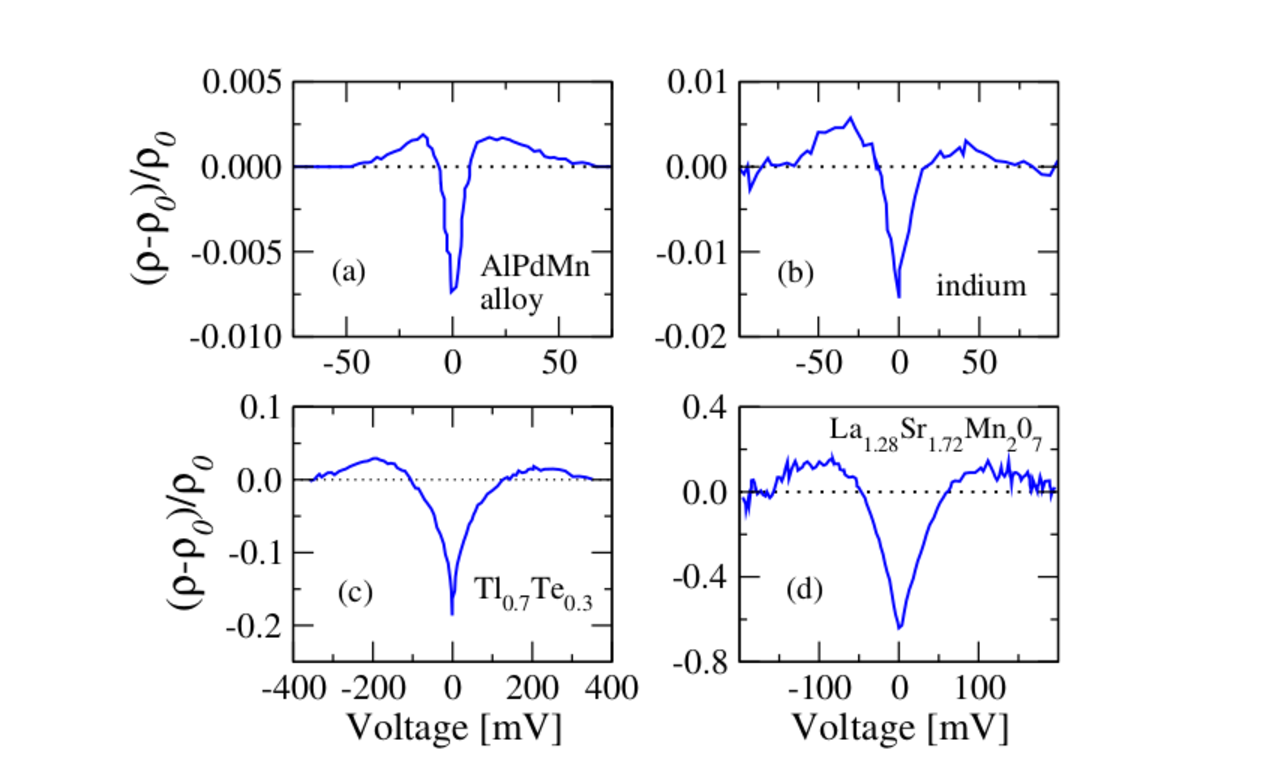
\includegraphics[scale=1]{grafy/B2}
\caption{Výsledky merania hustoty stavov tunelovou spektroskopiou pre rôzne kovy. Panel (d) ukazuje experimentálny výsledok z práce \cite{Mazur}. Dáta v paneloch (a), (b), a (c)
boli získané v práci \cite{Moskova} normovaním $G(|U|)$ závislostí nameraných v prácach \cite{Schmitz1}, \cite{Schmitz2}, \cite{Escudero}. V blízkom okolí Fermiho energie všetky ukázané spektrá vykazujú Altshuler-Aronovov jav $\rho(|\E- \E_F|) \propto \sqrt{|\E- \E_F|}$. Ďaleko od Fermiho energie už Altshuler-Aronovova závislosť
$\rho(|\E- \E_F|) \propto \sqrt{|\E- \E_F|}$ očividne neplatí a pre dostatočne veľké hodnoty $|\E - \E_F|$ vidno, že $\rho(|\E- \E_F|)$ s rastúcim $|\E - \E_F|$ klesá k $\rho_0$ zhora. }
\label{fig:B2}
\end{figure}



%%%KONIEC NOVEHO experimentalne %%%%%%%%%%%%%%%%%%%%%%%%%%%%
%%%%%%%%%%%%%%%%%%%%%%%%%%%%%%%

\newpage

